\documentclass[12pt]{article}
\usepackage{../../../assignment}
\usepackage{../../../math}
\usepackage{../../../uark_colors}
\hypersetup{
  colorlinks = true,
  allcolors = ozark_mountains,
  breaklinks = true,
  bookmarksopen = true
}

\newcommand{\answer}[1]{{\color{blue_winged_teal}\textbf{Answer:} #1}}
\newcommand{\pts}[1]{{\color{zinc500}[#1 points]}}

\begin{document}
\begin{center}
  {\Huge\bf Midterm - Fall 2026}

  \smallskip
  {\large\it ECON 5783 — University of Arkansas}
\end{center}

% {\fontsize{18}{24}\selectfont
\medskip
\begin{enumerate}
  \item Say a researcher wants to model the conditional expectation of annual earnings given gender, state of residence, and whether a worker has a college degree.
  They have a sample of 1,000 workers.
  Gender is recorded male and female, state of residence (50 states), and college degree is a binary indicator.
  \begin{enumerate}[label=(\alph*)]
    \item Describe how you would estimate this conditional expectation function ``fully flexibly''. 
    Use college-educated women in Arkansas as an example.

    \answer{
      We woudl estimate the conditional expectation function by taking sub-samples defined by $X_i = x$ and take sub-sample averages.
    }

    \item Why might this approach be impractical with this data?
    
    \answer{
      This is a classic example of the curse of dimensionality. 
      There are likely very few, if any, college-educated women in Arkansas in our sample of 1000 workers.
    }

    \item The researcher instead uses a linear model with an intercept, an indicator for being male, an indicator for having a college degree, and indicators for each of the 50 states (omitting a reference category for each variable).
    What does this model leave out relative to the fully flexible CEF?
    Give an example of a pattern in average earnings that this model would not be able to capture.

    \answer{
      This linear model has no interaction terms. 
      For example, perhaps the returns to college vary by what state you life in.
      Or, gender wage gaps differ by state. 
    }
  \end{enumerate}

  \newpage
  \item A researcher wants to estimate the returns to college using men in the National Longitudinal Survey of Young Men.
  The outcome is hourly wages in 1976, and treatment is completing at least 16 years of schooling.
  The table below compares average characteristics of men who attended and did not attend college (before any matching).
  The characteristics describe family background and where the men lived in 1966.

  % Source: wooldridge::card. Unweighted means among complete cases for
  % educ, wage, motheduc, fatheduc, momdad14, south66, and smsa66.
  % Treatment: educ >= 16. Differences are treated minus untreated.
  \begin{center}
    \begin{tabular}{lrrr}
      \toprule
      % & \multicolumn{2}{c}{Years of schooling} & \\
      & High School & College & Difference \\
      \midrule
      Mother's years of schooling & $9.98$ & $12.03$ & $2.15$ \\
      Father's years of schooling & $9.05$ & $11.94$ & $2.89$ \\
      Lived with both parents at age 14 & $0.933$ & $0.967$ & $0.034$ \\
      Lived in the South in 1966 & $0.359$ & $0.313$ & $-0.046$ \\
      \midrule
      Number of observations & 685 & 703 & \\
      \bottomrule
    \end{tabular}
  \end{center}

  \bigskip
  \begin{enumerate}[label=(\alph*)]
    \item What does this table tell you about the comparability of the two groups?
    Discuss at least two differences and explain which direction they would likely bias  the difference-in-means estimate.

    \answer{These two groups look very different. I think these estimates bias our estimated returns to schooling in the positive direction. For example, take parental education. College students tend to have more educated parents which likely has a positive impact on earnings.}

    \item The researcher decides to use nearest-neighbor matching on the four variables in the table.
    Describe in words the nearest-neighbor matching procedure. 
    You do not need to write a formula or code; just describe in words the steps that one would do.

    \answer{
      For each treated unit, find the control unit (say with replacement) whose $X$ values are closest to the treated unit, measured by the Mahalanobis distance.

      This forms a set of treated units and a set of matched control units. 
      From here, form a difference-in-means estimator using the treated and matched control group.
    }

    \item Instead of matching, the researcher might want to use a regression adjustment approach. 
    Describe in words the steps to implement this estimator. 
    You do not need to write a formula or code; just describe in words the steps that one would do.

    \answer{
      Using just untreated units, run a regression of $Y$ on the covariates. 
      This is our estimated model for $Y_i(0)$ as a function of $X_i$. 

      Take the fitted values $\hat{Y}_i(0)$ for the control units.
      Average $Y_i - \hat{Y}_i(0)$ over the treated units to form the treatment effect estimate.
    }
  \end{enumerate}
\end{enumerate}

\newpage
\noindent
% https://eml.berkeley.edu/~sdellavi/wp/FoxVoteQJEAug07.pdf
The following questions refer to ``The Fox News Effect: Media Bias and Voting'' by DellaVigna and Kaplan (2007).
The authors study whether making Fox News available on local cable affects voting.
By the 2000 presidential election, some towns had access to Fox News while others did not.

\medskip
\begin{enumerate}
  \setcounter{enumi}{2}
  \item Say a researcher compares the average Republican vote share in 2000 between towns with and without Fox News.
  Do you think this difference-in-means estimate identifies the causal effect of Fox News availability?
  Give a reason why the estimate might be biased, predict the sign of the bias, and explain your thinking.

  \answer{
    It is likely the case that Fox News did not roll out in a completely random fashion. 
    If there goal was to have a lot of viewers early on, they would likely target more Republican-leaning locations. 
    This would mean our difference-in-means estimate would conflate the effect of Fox News with preexisting differences in political alignment.
  }

  \medskip
  \item The authors present evidence that, conditional on geographic and cable-market controls, Republican vote share in 1996 did not predict whether a town had Fox News by 2000.
  Why might this be useful information for assessing the plausibility of the seleciton on observables assumption?
  Explain your thinking.

  \answer{
    This evidence suggests that prior to Fox News coming, there does not seem to be differences in baseline political ideology, after controlling for the controls.
    This makes it less likely that there are differences in unobservables between the treated and control (conditional on controls).
  }
\end{enumerate}

\newpage
\noindent
For the following questions refer to Figure \ref{fig:sat_rdd}.
These are two figures created using synthetic data.
The setup is that students in Michigan are guaranteed admission to the University of Michigan if they get at least a 1350 on their SAT.
Students, of course, are allowed to retake the SAT as many times as they want and the top score is used.
A researcher wants to estimate the effect of guaranteed admission on students' future earnings.

\medskip
\begin{enumerate}
  \setcounter{enumi}{4}
  \item Figure \ref{fig:sat_rdd}(a) presents the researcher's main result.
  What do we need to assume for the jump in future earnings at 1350 to identify the causal effect of guaranteed admission?
  % I am not looking for the `generic' assumption here; I want you to describe the assumption in the context of the research question.

  \answer{
    We need to assume that individuals who score just below the SAT cutoff look the same in terms of observables and unobservables to those just above the SAT cutoff.
    In practice, this means we can't have certain kinds of people choosing to retake until they get over the cutoff (`sorting').
  }

  \medskip
  \item Figure \ref{fig:sat_rdd}(b) shows average family income, measured before students take the SAT.
  Do you think this figure strengthens or weakens the researcher's causal claim?
  Explain how it relates to the assumption you discussed in the previous question.

  \answer{
    This figure weakens their causal claim since this is clear evidence of sorting along the cutoff. 
    It seems like families with higher income were more likely to retake the SAT to make it above the cutoff.
    This is a form of selection bias that will bias our RDD estimate (conflating family income with the effect of the policy).
  }

  \medskip
  \item The researcher responds by using only students with SAT scores very close to 1350.
  Do you think using a smaller bandwidth fixes the concern you described above?
  Why or why not?

  \answer{
    No, a smaller bandwidth does not fix the problem. 
    This is because our continuity assumption is not valid, so no matter how close we get to the cutoff, there are differences in $Y(0)$ between the treated and control units.
  }
\end{enumerate}

\medskip
\begin{figure}[htb!]
  \caption{Simulated Data}
  \label{fig:sat_rdd}
  \begin{center}
    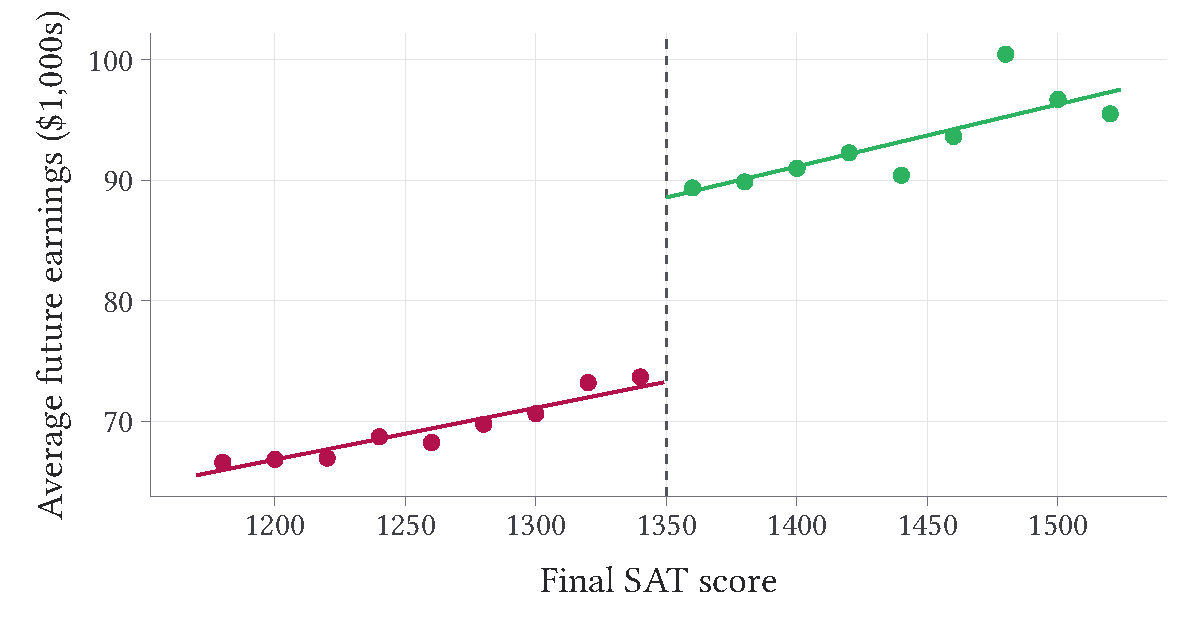
\includegraphics[width = 0.8\textwidth]{sat_sorting_earnings.pdf}
    \subcaption{RDD Estimate on Student's Future Earnings}
  \end{center}

  \begin{center}
    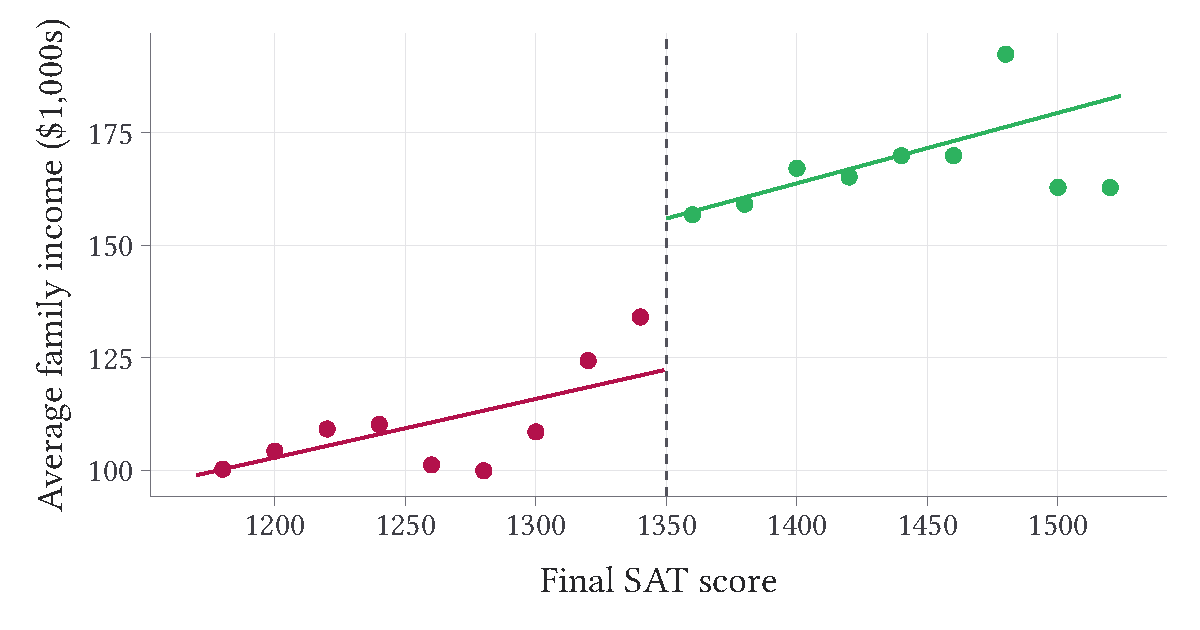
\includegraphics[width = 0.8\textwidth]{sat_sorting_family_income.pdf}
    \subcaption{RDD Estimate on Family Income}
  \end{center}
\end{figure}
% }

\end{document}
